\section{Cellular Security}


\subsection{1G: Analog}

\paragraph{Overview}
Introduced in the early 1980s to connect to the telephone network (\textit{Public Switched Telephone Network PSTN}).
Medium access control: split bandwidth with FDMA, with one call using the same frequency in both directions.
Suppprts handover between different base stations.

\paragraph{No security}
Identification via serial and phone numbers.
Control messages as analogue tones.

\underline{Problems:} eavesdropping (privacy), mobile cloning (billing fraud).


\subsection{2G: GSM}

\paragraph{Overview}
Introduced in the early 1990s.
Digital voice and control messages, enabling features like: compression, error correction, less power, SMS, security mechanisms.
We focus on the \textit{Global System for Mobile Communications GSM}.

\paragraph{Architecture}
See \autoref{fig:2g-arch}.

Medium access control: FDMA with distinct uplink/downlink frequency channels.
TDMA\footnote{Time-division multiple access} to support 8 speech channels on the same frequency.

Different channels for traffic and control frames (e.g. paging channel, random access channel, access grant channel).

\begin{figure}[h]
	\centering
	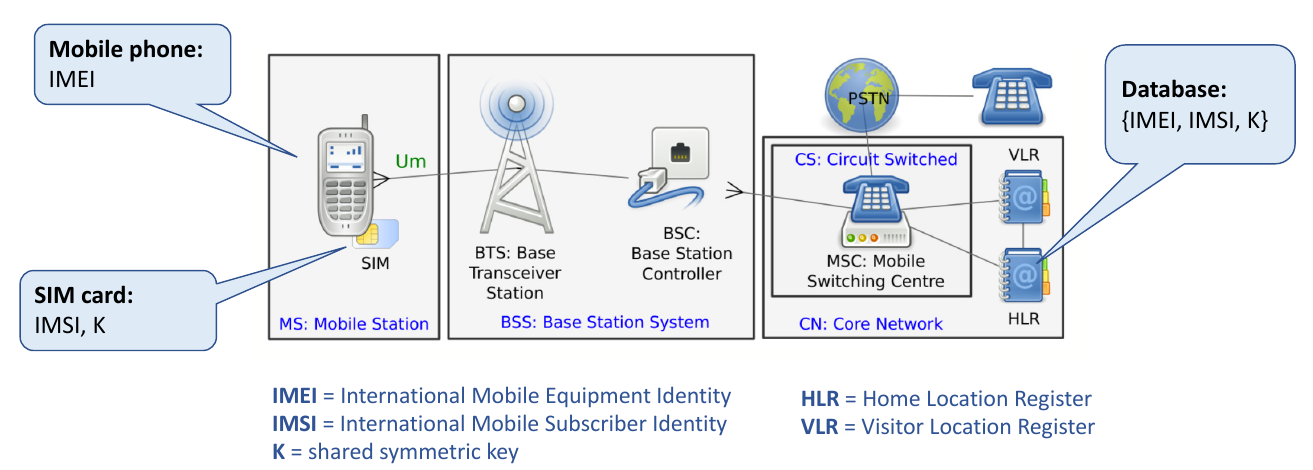
\includegraphics[scale=0.45]{images/10-2g-arch.png}
	\caption{Architecture of 2G}
	\label{fig:2g-arch}
\end{figure}

\begin{figure}
	\centering
	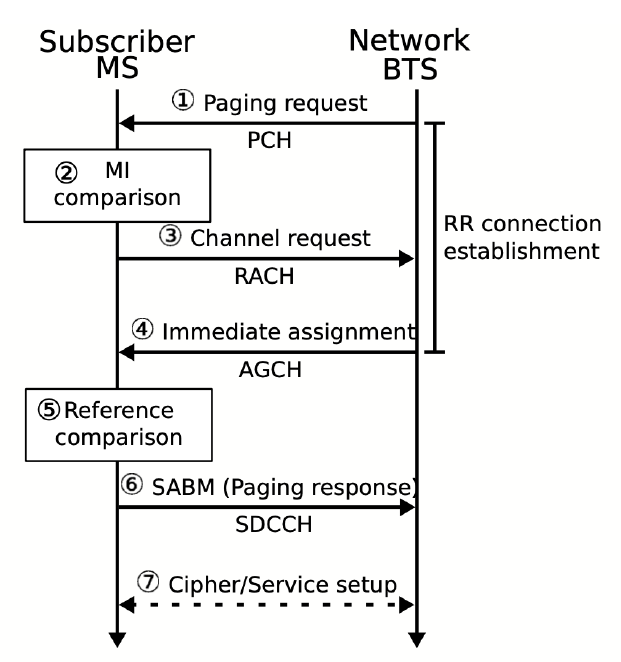
\includegraphics[scale=0.4]{images/10-2g-channels.png}
	\caption{Setup of incoming call (BTS ``pages'' the MS) over the different channels}
	\label{fig:2g-channels}
\end{figure}

\paragraph{Security model}
Everything based on symmetric shared keys $K_i$.
The key is stored in the \textit{Home Location Register HLR} of the provider and on the \textit{subscriber identification module SIM} card (and never leaves it).

\underline{Algorithms:}
A3 for authentication, A5 for encryption, A8 for key derivation.
Initially secret, but e.g. A5 leaked in the mid 90s, reverse engineered in 1999.

\paragraph{GSM authentication}
See \autoref{fig:2g-authentication}.
From the shared key $K_i$ and a random challenge a session key $K_c$ is derived.
Together with the frame nonce/counter $F_n$ it is used to encrypt the plaintext frame $m_i$.

Note that there is no mutual authentication (only the phone is authenticated) and messages can be replayed!
Also note that since A3 and A8 are executed on the SIM card, the operator can choose these!

\begin{figure}
	\centering
	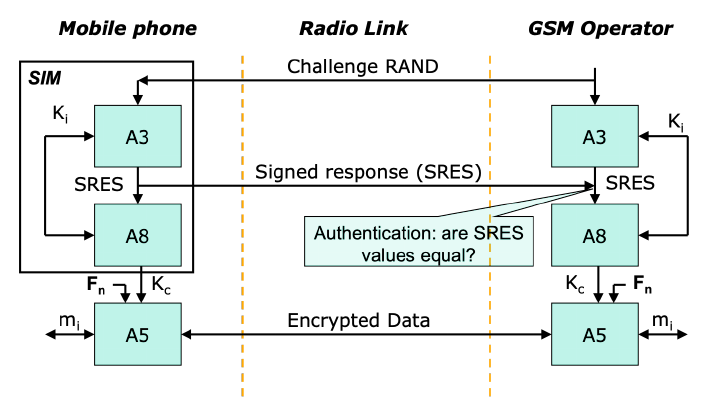
\includegraphics[scale=0.5]{images/10-2g-authentication.png}
	\caption{2G (Authentication) Flow}
	\label{fig:2g-authentication}
\end{figure}

\paragraph{GSM encryption}
Goal: fast in hardware.
Two variants A5/1 (strong) and A5/2 (weak, not discussed here).

\underline{A5/1:} stream cipher with a \textit{Linear Shift Feedback Register LSFR} and 64 bit security.
Registers are initialised with the key $K_c$ and the frame counter $F_n$ to create the keystream, which is then XORed with the plaintext.
See \href{https://web.archive.org/web/20120326211404/http:/l-system.net.pl/crypto/A5\_1\_stream\_cipher.svg}{here} for a visualisation of the LSFR.

\underline{Attack approach:} \\
Known plaintext/ciphertext pair
$\overset{XOR}{\longrightarrow}$ keystream
$\longrightarrow$ secret internal state
$\overset{solve\; LSE\; with\; 64\; eqns}{\longrightarrow}$ key

\begin{figure}
	\centering
	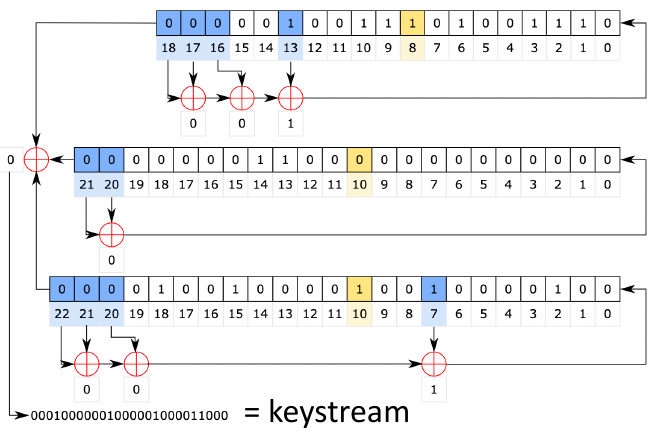
\includegraphics[scale=0.5]{images/10-2g-a5.png}
	\caption{2G A5 Linear Shift Feedback Registers}
	\label{fig:2g-a5}
\end{figure}

\paragraph{A5/1 attacks}
Attacks of A5/1 evolved over time (2000--2010).
The first were not very practical (requiring many known plaintexts or special-purpose hardware).
Types included: Time-Memory Tradeoff Attack (Biryukov 2000, Nohl 2010), Correlation Attack (Brakan \& Birham 2005), Guess and Determine Attack (Gendrullis et al. 2008), Fast Near Collisions (Zhang 2019).
\\
Note that a few known plaintexts are reasonable (known control frames).

\href{https://media.blackhat.com/bh-us-10/whitepapers/Nohl/BlackHat-USA-2010-Nohl-Attacking.Phone.Privacy-wp.pdf}{\underline{Karsten Nohl (2010):}}
2TB precomputed table (mapping from keys/state to keystreams, 1 month computation with 4 GPUs), 64 bit plaintext, 5 sec attack time (lookup).%
\footnote{Nohl omitted some attack details, later provided by Lu (2015).}
\\
Challenge: reducing table size ($2^{64}$ unreasonable).

\paragraph{Time-Memory Tradeoff Attack} (Hellman 1980)
\begin{enumerate}
	\item Precompute chains $x_1 \overset{f}{\rightarrow} x_2 \overset{f}{\rightarrow} x_3 \overset{f}{\rightarrow} ...$ where $f$ is A5/1.
	Store start point SP and end point EP.
	\item Attack: Create chain for the observed keystream.
	Check if any element in the chain matches a known EP.
	Re-create chain from SP to find the likely key (the element before the keystream in the re-computed chain).
\end{enumerate}
Tradeoff: longer chains mean less storage but more computation during the attack.

\begin{figure}
	\centering
	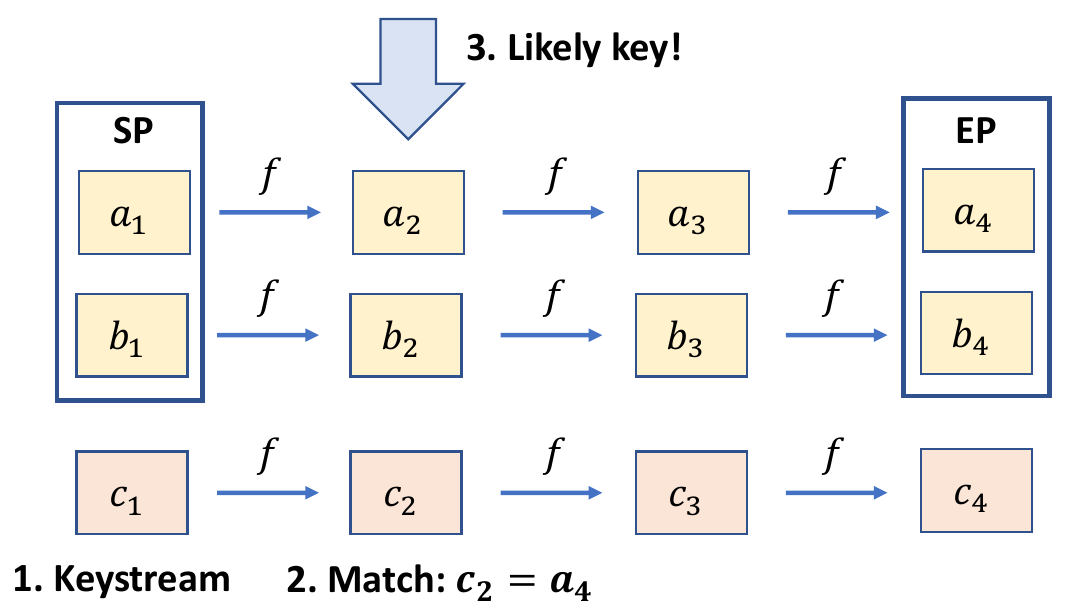
\includegraphics[scale=0.3]{images/10-2g-tmto.png}
	\caption{Time-Memory Tradeoff Attack}
	\label{fig:2g-tmto}
\end{figure}

\paragraph{Rainbow tables} (Oechslin 2003)
\\
Solves issue of collisions in chains (leading to reduced keyspace coverage as chains merge).
Uses different variant $f_i$ (``color'') for each chain link.
Different lookup details, but same idea.

\paragraph{A5/1 attacks summary}
Previous ideas generally applicable to stream ciphers, not just to A5/1.
Main enabler is the short key size (64 bit).
Nevertheless it lasted quite well considering when it was designed and under which hardware constraints, and given that there is still ongoing research.

\paragraph{A8 attacks}
Setup: $K_c$ known, want to recover $K_i$.
\\
1998: COMP128 hash inverted in hours (effectively only 54 bit)\\
2002: Faster recovery using side-channels.
\\
Mitigation: Operators replace A8 (OTA update, new SIM).

\paragraph{GSM -- no integrity protection}
No integrity protection defined, due to too much overhead (voice frame has 144 bits).
Also special use case: dropping frames/retransmission is undesired, and small voice frame modifications are acceptable.

\paragraph{GSM -- no mutual authentication}
Recall that the phone does not authenticate the base station.
Probable reasoning (1980s): expensive equipment, call encrypted anyway.
But: commercial fake BS (2000s), USRP (2010), etc enable user identification + tracking and MITM.


\subsection{SS7}

\paragraph{Signalling System 7 (SS7)}
Signalling network used in GSM + 3G to route calls, coordinate roaming, deliver SMS, etc.
Defined in the 80s/90s.

Initially only a few participating, mutually trusted operators.
But: Soon grew to 1000+ operators and third-party service providers, and SS7 access could be purchased at a low price.\\
$\implies$ Trust assumption violated.

Open source software and specs online, anybody with network access can send SS7 commands with a Linux computer.\\
$\implies$ Assumption on expensive equipment violated.

Attacks in 2014 by Engel (see the \href{https://media.ccc.de/v/31c3\_-\_6249\_-\_en\_-\_saal\_1\_-\_201412271715\_-\_ss7\_locate\_track\_manipulate\_-\_tobias\_engel}{31C3 talk here}), discussed below.

\begin{figure}
	\centering
	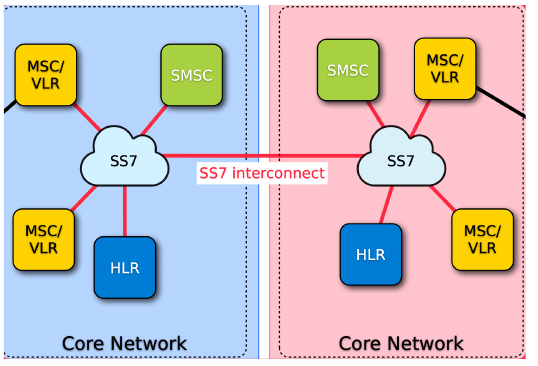
\includegraphics[scale=0.5]{images/10-ss7.png}
	\caption{SS7 Architecture}
	\label{fig:ss7}
\end{figure}

\paragraph{Location tracking}
Phone locations are stored in the \textit{Gateway Mobile Location Center GMLC}, access to which requires authentication (e.g. law enforcement).
However, by requesting the routing info from the HLR and with that the cell id from the \textit{Mobile Switching Center MSC} where the user is currently logged in, one can work around this to still get a rough location.

\begin{figure}
	\centering
	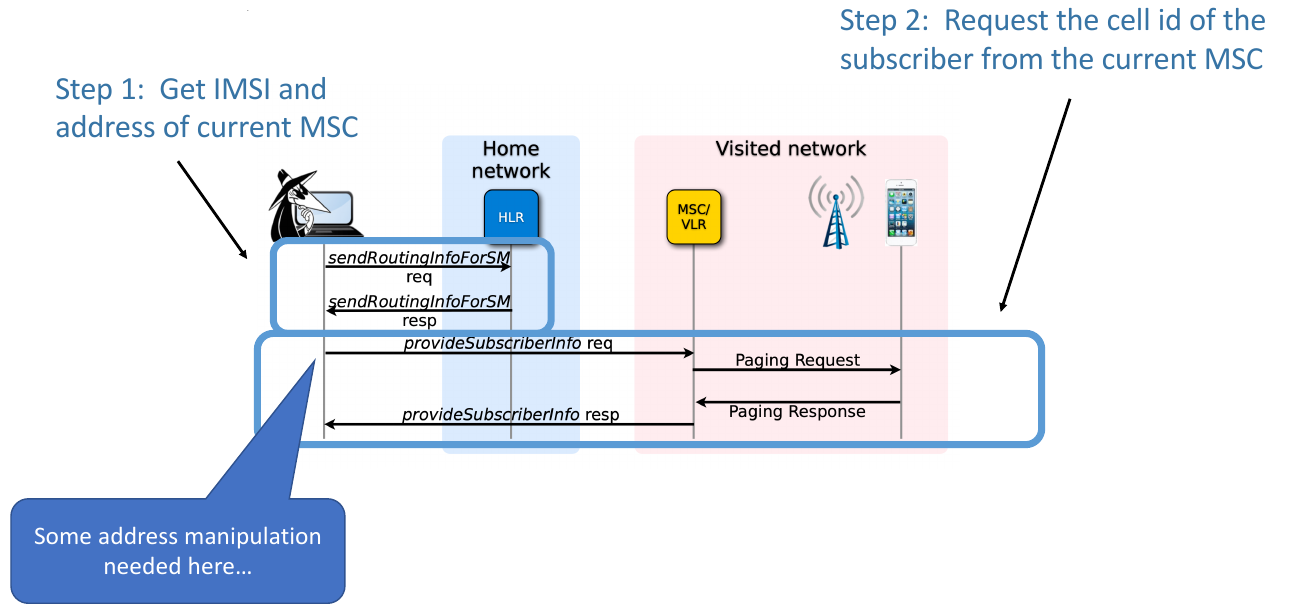
\includegraphics[scale=0.4]{images/10-ss7-location.png}
	\caption{SS7 Location Tracking}
	\label{fig:ss7-location}
\end{figure}

\paragraph{Intercepting Calls}
See \autoref{fig:ss7-calls}.
\begin{enumerate}
	\item Attacker overrides the \textit{GSM Service Control Function (gsmSCF)} in the MSC with their own.
	\item When the target makes a call, the MSC now contacts the attacker.
	\item The attacker learns the phone number and rewrites it towards their recording proxy.
	\item MSC sets up call to the proxy.
	\item Proxy bridges call to the intended receiver.
\end{enumerate}

\begin{figure}
	\centering
	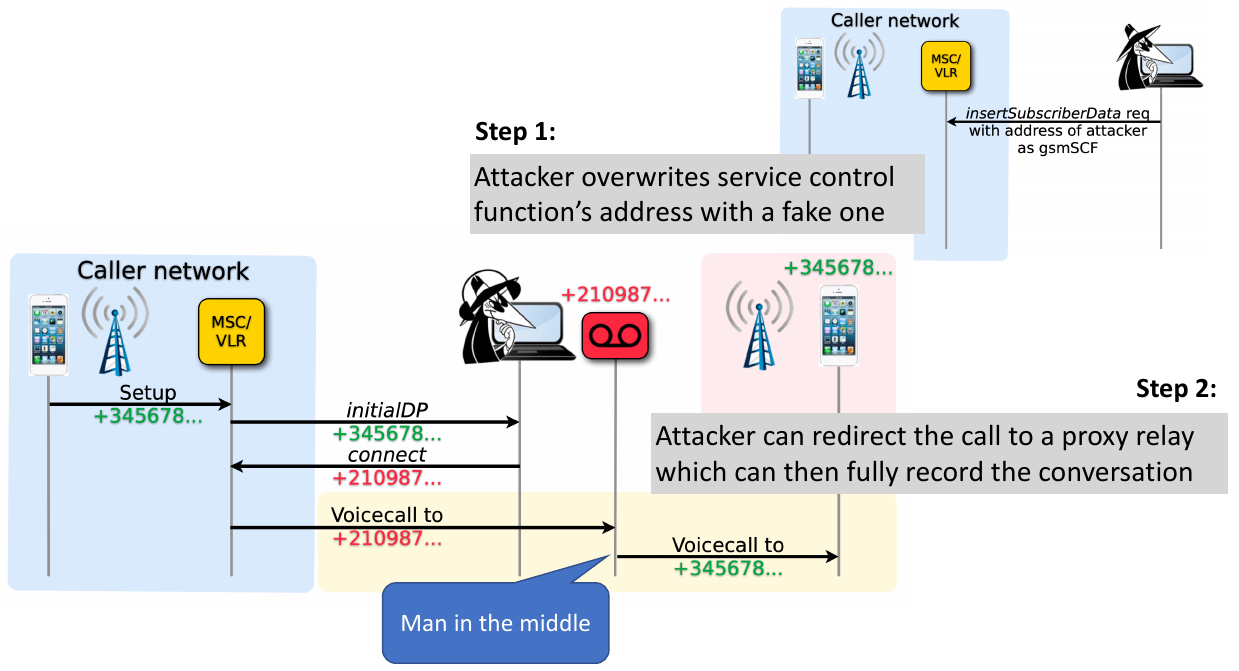
\includegraphics[scale=0.4]{images/10-ss7-calls.png}
	\caption{SS7 Intercepting Calls}
	\label{fig:ss7-calls}
\end{figure}

\paragraph{SS7 Summary}
Legacy system with outdated trust model.
Bad network management (open interfaces, no authentication or access control to control messages).
Attacks are independent of cryptography and the radio link (i.e. work from far away).
\\
Some issues were fixed, and LTE has a new signalling system (Diameter).


\subsection{3G: UMTS}

\paragraph{Overview}
\textit{Universal Mobile Telecommunication System UMTS} introduced in the early 2000s.

Radio link uses \textit{wideband code-division multiple access W-CDMA}, separate per-user spreading codes, distinct uplink and downlink frequency bands.

\paragraph{Protocol}
New \textbf{authentication and key agreement (AKA)} protocol.
Provides mutual authentication, mutual replay protection, integrity protection.
Also used in 4G+5G (more or less).

Similar design principles like GSM: operator and SIM trusted, phone and visited networks untrusted, minimise communication with home network.

\underline{Remarks:} (see \autoref{fig:3g-aka-details})
\begin{enumerate}
	\item Both the SIM card and the operator maintain the sequence number SQN (against replays)
	\item The IMSI\footnote{International Mobile Subscriber Identity} is send before the authentication (enabling tracking, see later)
	\item Function $f_1, f_2, f_3, f_4, f_5$ are operator-specific
	\item Loose synchronisation required
	\item Integrity key IK for integrity protection
\end{enumerate}

Further details on the authentication, encryption and integrity protection%
\footnote{Mandatory for signalling + control messages, optional for data. Based on a 8-round Feistel network to be fast in hardware.}
functions can be found in the slides but are omitted in this summary.

\begin{figure}
	\centering
	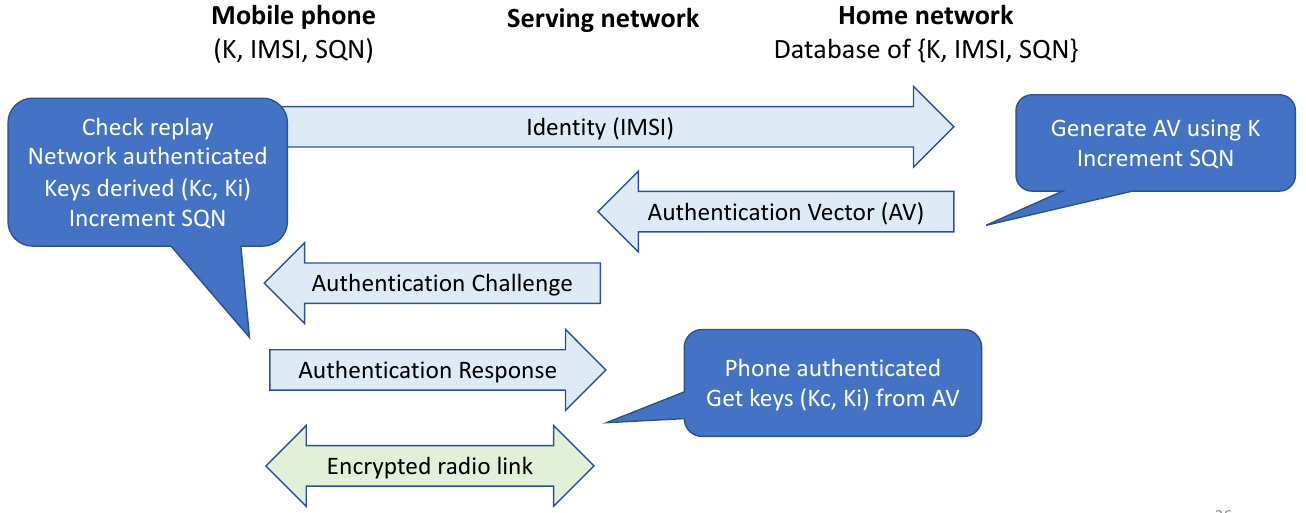
\includegraphics[scale=0.4]{images/10-3g-aka-overview.png}
	\caption{AKA High Level Flow}
	\label{fig:3g-aka-overview}
\end{figure}

\begin{figure}
	\centering
	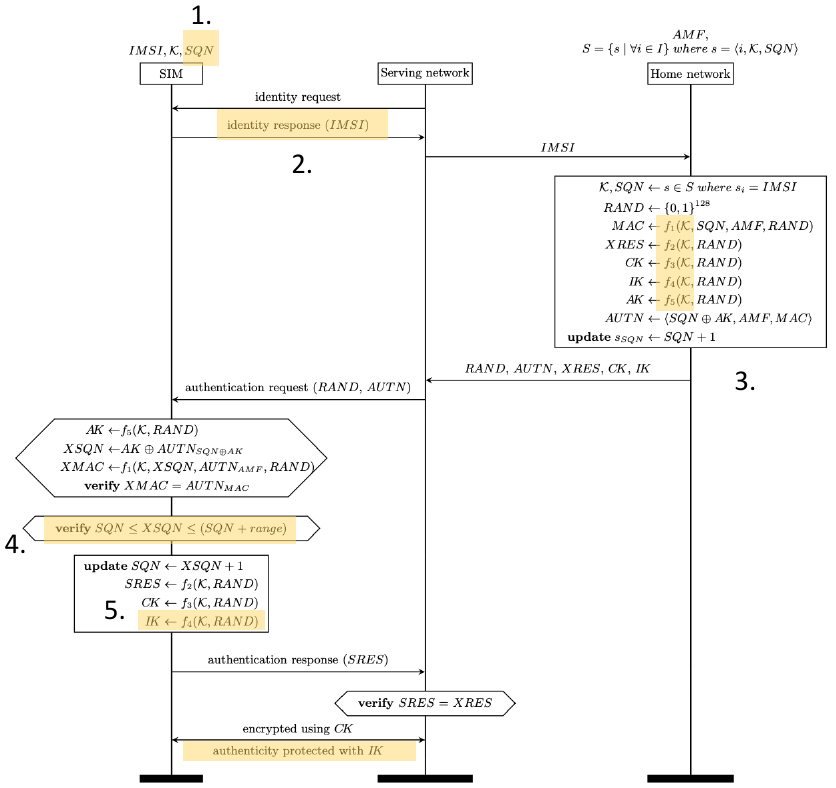
\includegraphics[scale=0.7]{images/10-3g-aka-details.png}
	\caption{AKA Detailed Flow}
	\label{fig:3g-aka-details}
\end{figure}

\paragraph{Cryptography Summary}
Authentication and Key Agreement protocol formally verified with respect to authentication and confidentiality (2001).
Two known but impractical attacks on encryption (interesting for research though).
TLDR: Good for now.

\paragraph{Denial of Service}
Commercial jammers available for a few hundred dollars (though use is illegal!).
\\
Approaches:
\begin{itemize}
	\item Insert noise on physical layer.
	\item Jam/block paging messages (control layer). Difficult, requires synchronisation with the victim.
	\item Answer paging messages faster than the victim, causing the victim's reply to be ignored.
	Possible because (a) paging occurs before authentication and (b) base stations cover large areas.
\end{itemize}

\paragraph{MITM/Fake BS}
Though AKA authentication is mutual, a MITM perform a downgrade attack to force the phone to use GSM (due to co-existence).
Also in 3G the MITM can learn the IMSI at the start of AKA.

\underline{Practical considerations:}
Which frequency to use -- allocated or unallocated?
What cell id to use -- a new, unknown one?
Jam legitimate BS to get victims to connect to yours?
\\
$\implies$ Though setting up a fake BS is easy, detecting it is easy as well.

\paragraph{Femtocells}
Operator provides a ``mini-BS'' to customers to improve local (indoor) coverage.
The femtocell box relays from the radio link to the operator network.

Vulnerable because they are easier to access then normal base stations (high up on a tower).
Gaining access gives a perfect MITM position, having the keys for the gateway to the operator as well as for the radio link.

\paragraph{User tracking}
Identity (IMSI) is sent before authentication.
Even though a temporary identity (IMSI) is issued, the IMSI is reused on occasions.
Thus user tracking is possible to some extent, but not addressed by the spec (tradeoff possibility of abuse versus increased complexity).

\underline{Approaches for identity protection}:
\begin{itemize}
	\item \textit{Pseudonyms}: send pseudonym when starting AKA, with the home network always returning a new pseudonym
	(encrypted\footnote{Note that this encryption can be done symmetrically with the shared key, since the home network could use the pseudonym to look it up.}, so that the serving network cannot read it).\\
	Challenge: requires synchronisation, and thus a recovery process.
	However, it is hard to design a recovery process that cannot be abused to learn the IMSI.
	\item \textit{Public key encryption}: store home network public key on SIM, encrypt IMSI.
	Defined as optional in 5G.
	Pro: no state that needs to be synchronised.
	Con: asymmetric cryptography is expensive.
\end{itemize}


\subsection{4G: LTE}

\paragraph{Overview}
\textit{Long-Term Evolution LTE} introduced in 2008.
\\
\underline{Updated architecture:}
fully packet switched, new core network (\textit{Evolved Packet Core EPC}, fully packet-switched), new radio network (\textit{Evolved UMTS Terrestrial Radio Access Network E-UTRAN}), but interoperable with legacy systems.
\\
\underline{Updated physical layer:}
\textit{Orthogonal Frequency Division Multiplexing OFDM} (downlink with orthogonal sub-carriers, single-carrier uplink), multiple antennas (MIMO).

\paragraph{Architecture and Terminology}
See \autoref{fig:4g-arch}.
\begin{itemize}
	\item \textit{User Equipment UE} (MS): the mobile handset
	\item \textit{Evolved Node B eNB} (BS): the base station
	\item \textit{Mobility Management Entity MME}: handles signalling via the \textit{Non-access stratum NAS}, UE authorisation, S-GW selection
	\item \textit{Home Subscriber Server HSS} (HLR): subscriber database, user authentication
	\item \textit{Serving Gateway S-GW}:  routes user data packets
	\item \textit{Packet Gateway P-GW}: connects to external network, routing, filtering
\end{itemize}

\begin{figure}
	\centering
	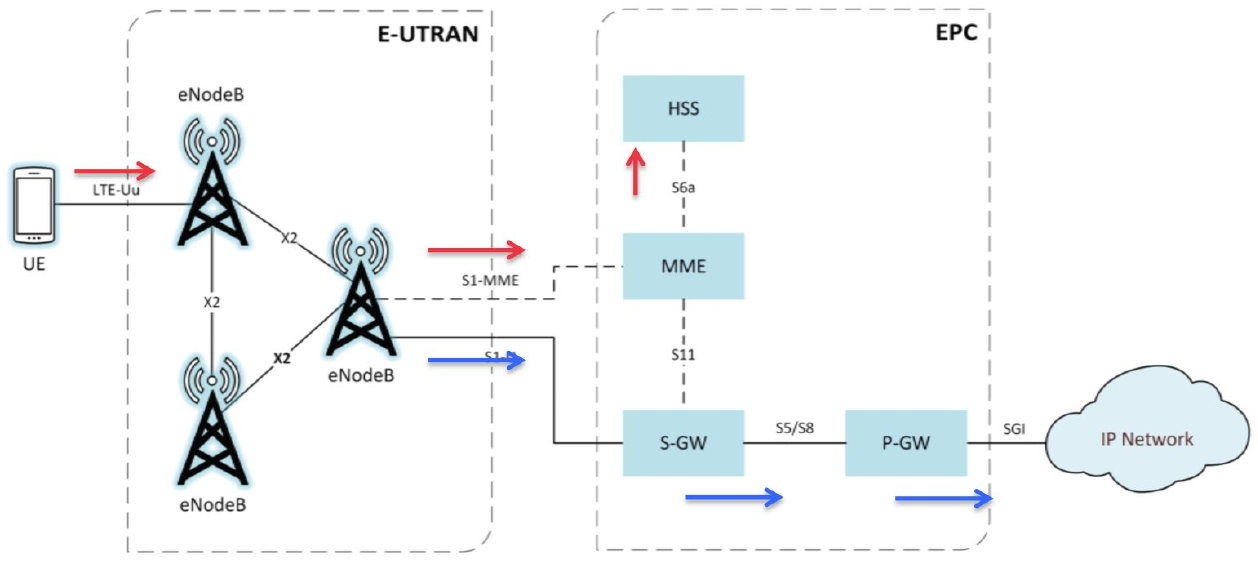
\includegraphics[scale=0.5]{images/10-4g-arch.png}
	\caption{LTE Architecture}
	\label{fig:4g-arch}
\end{figure}

\paragraph{Network Protocol Stack}
See \autoref{fig:4g-network-stack}. From top to bottom:
\begin{itemize}
	\item \textit{Non-access stratum NAS}: mobility management, tracking area update, etc
	\item \textit{Radio Resource Control RRC}: AKA, paging messages, system information broadcast, etc.
	\item \textit{Packet Data Convergence Protocol PDCP}: compression, optionally encryption+integrity
	\item \textit{Radio Link Control RLC}: error correction, segmentation, frame ordering
	\item \textit{MAC layer}: manages access to radio link
\end{itemize}
Note that everything below the PDCP layer is unencrypted.
Thus most sniffing+spoofing attacks focus on the layers below.

\begin{figure}
	\centering
	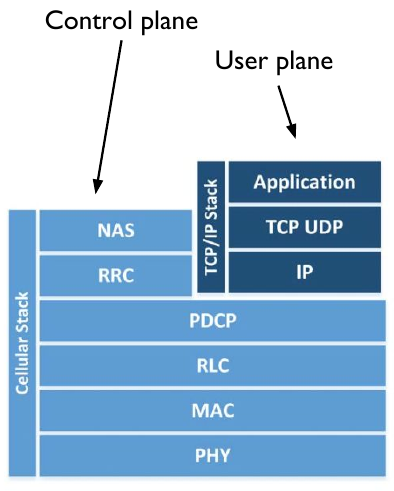
\includegraphics[scale=0.5]{images/10-4g-network-stack.png}
	\caption{LTE Network Protocol Stack}
	\label{fig:4g-network-stack}
\end{figure}

\paragraph{Security Overview}
Authentication: similar to AKA.

Encryption/integrity: 3 variants EEA1, EEA2, EEA3 and EIA1, EIA2, EIA3.

Other: extended key hierarchy, option for longer keys (256 bit), handover between eNBs (X2), backhaul (S1) protection.

\paragraph{Key hierarchy}
to limit attack possibilities and impact.
Master key $K$ (128 bits, stored on HSS+SIM), confidentiality key $CK$, integrity key $IK$, etc.
\begin{figure}
	\centering
	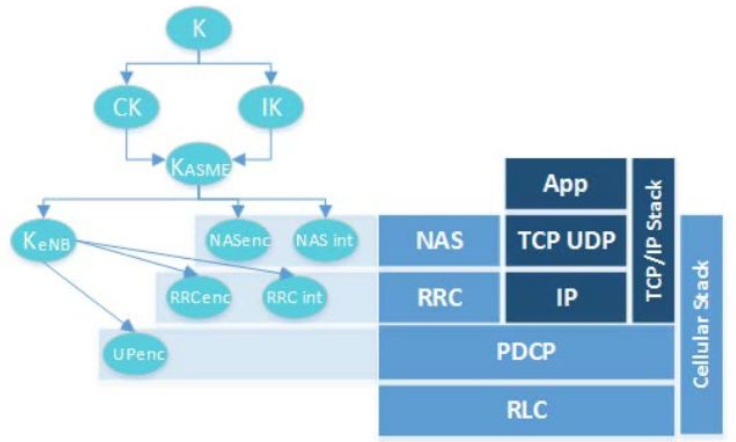
\includegraphics[scale=0.5]{images/10-4g-key-hierarchy.png}
	\caption{LTE Key Hierarchy}
	\label{fig:4g-key-hierarchy}
\end{figure}

\paragraph{Backhaul + EPC protection}
For backhaul, the LTE spec recommends physical protection.
For EPC, the spec is vague (``division of security domains'').
In practice both are secured using standard IP security practices (VPN, PKI).

\paragraph{Handover + Key Separation}
Reduced attack surface and key scope by limiting key lifetime of $K_{eNB}$.
E.g. different keys for different eNBs/cells.

\paragraph{Location tracking} \mbox{} \\
\underline{Background:}
The service area is divided intro \textit{tracking areas TAs} containing multiple cells (each controlled by an eNodeB that broadcasts information such as the TA code, mobile network code, cell ID).
UE sends IMSI with the Attach request, in which the operator assigns temporary identifiers that are used subsequently (TMSI, GUTI\footnote{Global unique temporary identifier}).

\underline{Adversary:}
Goal: learn user locations.
Capabilities: transmit/receiver radio signals, possible with commercial USRPs.
Advantage: GUTI re-allocation depends on operator, possibly not changed for multiple day.

\underline{Attack:}
\begin{enumerate}
	\item Set up fake BS.
	\item Monitor user presence in TA.
	\item Learn precise location:
	actively send unprotected \textit{RRC Connection Reconfig} messages, to which the UE responds with a \textit{Measurement Report} containing the signal strengths of neighbouring cells and its GPS location.
\end{enumerate}

\underline{Analysis:}
Not all signalling/control messages are integrity protected/authenticated.
Spec allows this explicitly for troubleshooting (availability versus privacy).

\paragraph{MITM} \mbox{} \\
\underline{Background:}
MAC layer assigns unique \textit{Radio Network Temporary Identifiers RNTIs} to distinguish UEs.
eNodeB uses \textit{Downlink Control Information DCI} to notify UEs when radio resources are available.
Also recall that EEA2 uses AES-CTR for encryption (XORs keystream with plaintext).

\underline{Attack:}
\begin{enumerate}
	\item Identify UE from encrypted traffic: observe connection establishment, learn TMSI+RNTI, use paging to map TMSI to phone number.
	\item Modify/redirect encrypted traffic: often uplink is encrypted but not integrity protected. Xor ciphertext with ``manipulation mask'' (try-and-error).
\end{enumerate}

\underline{Analysis:}
Identifiers on lower layers, encryption on higher layers.
Integrity protection optional.

\paragraph{Jamming/DoS}
Brute-force jamming always possible, but requires a lot of power.
Instead, targeting specific control channels can be effective, too (see next point).

\paragraph{Signal Overshadowing (SigOver)} \mbox{} \\
\underline{Idea:}
Broadcast signals are not integrity protected (e.g. \textit{System Information Blocks SIBs)}.
Spoof them by overshadowing specific frames of the legitimate broadcasts (providing a misconfiguration to prevent the UE from connecting).

\underline{Analysis:}
Low jamming-to-signal ratio (J/S), thus stealthy (not as obvious as a fake BS).
Only downlink affected, thus undetected by the base station.
Challenges: time+frequency synchronisation with the legitimate signal, distance/delay estimation to the UE, phone may quickly reconnect to another cell.

\underline{Commercial Mobile Alert Service CMAS} messages (``presidential alerts'') are also delivered via SIB12, allowing signal overshadowing.

\paragraph{Keystream Reuse Attack / ReVoLTE} \mbox{} \\
\underline{Idea:} IV for EEA comprised of a counter, radio bearer ID and radio direction.
\\
Unfortunately, many operators re-use bearer IDs and reset counter for subsequent calls (exactly what we need!).
Adversary can initiate a second call just after the target call and record both keystreams.
\\
Fix: don't repeat id and counter.

\paragraph{4G Summary}
New crypto algorithms, new core network.
Small security improvements (key hierarchy, handover protection), but not yet perfect.
\\
Types of attacks: SigOver, fake base stations, man-in-the-middle.
\\
Attack properties: stealthiness/detectability, power requirement, J/S ratio.


\subsection{5G}

\paragraph{Overview}
Currently being deployed (2019/2020).
\\
\underline{Radio link}: \textit{5G New Radio NR}, optimised OFDM, massive MIMO, two frequency ranges (FR1: sub-6GHz, FR2: mmWave range, 24-100GHz, high-throughput, high-bandwidth).
Beam management to steer beams with a phase array allows connecting more devices.
\\
\textit{Time Division Duplex TDD} allows the same channel/frequency to be used for both up- and downlink, with different time intervals for different directions.%
\footnote{Compare this with LTE which used FDD: the uplink and downlink used different frequencies.}
On one hand this allows flexible allocation, but on the other it requires precise synchronisation!

\paragraph{Attacks}
Some ideas as research is ongoing.
\begin{itemize}
	\item Beam stealing: attack beam training to steer beams away from victims (shown for IEEE 802.11ad)
	\item Broadband jamming (DoS): increasingly difficult due to large bandwidth (power constraint) $\implies$ need protocol-aware spoofing for DoS (challenge: tight synchronisation).
	\item PSS\footnote{Primary Synchronisation Signal} spoofing:
	soft takeover: synchronise to cell, introduce PSS at correct timing then slowly move peak away (see GNSS \autoref{sec:gps-spoof}).
\end{itemize}

\paragraph{5G Security Summary}
Similar crypto algorithms.
Better replay protection for AKA (SIM generates nonces).
User tracking mitigations (SIM can encrypt IMSI/TMSI with home operator's public key, stricter policies for changing temporary ids).

\begin{figure}[h]
	\centering
	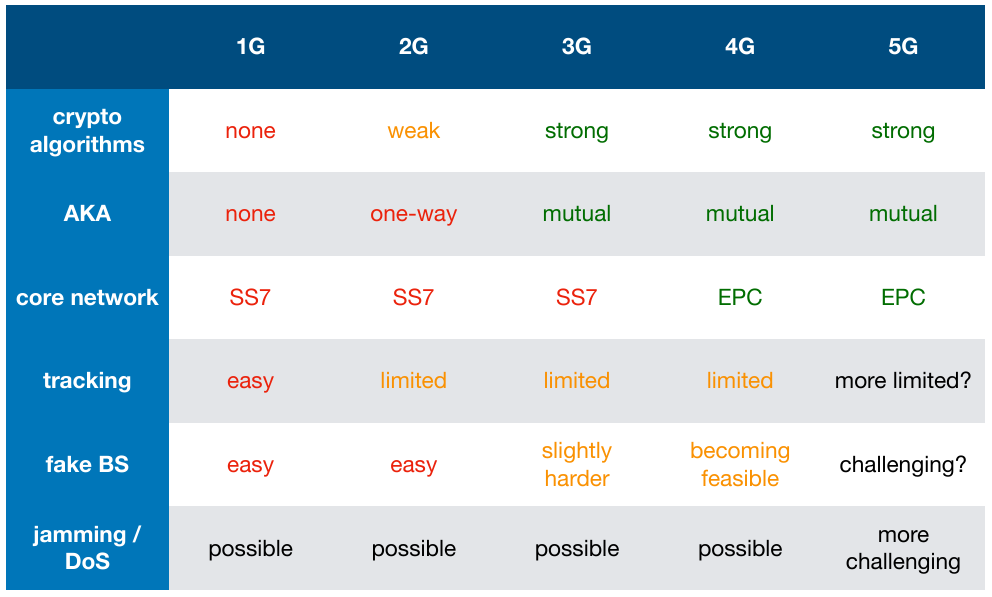
\includegraphics[scale=0.5]{images/10-overview.png}
	\caption{Cellular Security Summary}
	\label{fig:overview}
\end{figure}

